% Options for packages loaded elsewhere
\PassOptionsToPackage{unicode}{hyperref}
\PassOptionsToPackage{hyphens}{url}
%
\documentclass[
  english,
  man, fleqn, noextraspace,floatsintext]{apa6}
\title{The title}
\author{First Author\textsuperscript{1} \& Ernst-August Doelle\textsuperscript{1,2}}
\date{}

\usepackage{amsmath,amssymb}
\usepackage{lmodern}
\usepackage{iftex}
\ifPDFTeX
  \usepackage[T1]{fontenc}
  \usepackage[utf8]{inputenc}
  \usepackage{textcomp} % provide euro and other symbols
\else % if luatex or xetex
  \usepackage{unicode-math}
  \defaultfontfeatures{Scale=MatchLowercase}
  \defaultfontfeatures[\rmfamily]{Ligatures=TeX,Scale=1}
\fi
% Use upquote if available, for straight quotes in verbatim environments
\IfFileExists{upquote.sty}{\usepackage{upquote}}{}
\IfFileExists{microtype.sty}{% use microtype if available
  \usepackage[]{microtype}
  \UseMicrotypeSet[protrusion]{basicmath} % disable protrusion for tt fonts
}{}
\makeatletter
\@ifundefined{KOMAClassName}{% if non-KOMA class
  \IfFileExists{parskip.sty}{%
    \usepackage{parskip}
  }{% else
    \setlength{\parindent}{0pt}
    \setlength{\parskip}{6pt plus 2pt minus 1pt}}
}{% if KOMA class
  \KOMAoptions{parskip=half}}
\makeatother
\usepackage{xcolor}
\IfFileExists{xurl.sty}{\usepackage{xurl}}{} % add URL line breaks if available
\IfFileExists{bookmark.sty}{\usepackage{bookmark}}{\usepackage{hyperref}}
\hypersetup{
  pdftitle={The title},
  pdfauthor={First Author1 \& Ernst-August Doelle1,2},
  pdflang={en-EN},
  pdfkeywords={keywords},
  hidelinks,
  pdfcreator={LaTeX via pandoc}}
\urlstyle{same} % disable monospaced font for URLs
\usepackage{graphicx}
\makeatletter
\def\maxwidth{\ifdim\Gin@nat@width>\linewidth\linewidth\else\Gin@nat@width\fi}
\def\maxheight{\ifdim\Gin@nat@height>\textheight\textheight\else\Gin@nat@height\fi}
\makeatother
% Scale images if necessary, so that they will not overflow the page
% margins by default, and it is still possible to overwrite the defaults
% using explicit options in \includegraphics[width, height, ...]{}
\setkeys{Gin}{width=\maxwidth,height=\maxheight,keepaspectratio}
% Set default figure placement to htbp
\makeatletter
\def\fps@figure{htbp}
\makeatother
\setlength{\emergencystretch}{3em} % prevent overfull lines
\providecommand{\tightlist}{%
  \setlength{\itemsep}{0pt}\setlength{\parskip}{0pt}}
\setcounter{secnumdepth}{-\maxdimen} % remove section numbering
% Make \paragraph and \subparagraph free-standing
\ifx\paragraph\undefined\else
  \let\oldparagraph\paragraph
  \renewcommand{\paragraph}[1]{\oldparagraph{#1}\mbox{}}
\fi
\ifx\subparagraph\undefined\else
  \let\oldsubparagraph\subparagraph
  \renewcommand{\subparagraph}[1]{\oldsubparagraph{#1}\mbox{}}
\fi
\newlength{\cslhangindent}
\setlength{\cslhangindent}{1.5em}
\newlength{\csllabelwidth}
\setlength{\csllabelwidth}{3em}
\newlength{\cslentryspacingunit} % times entry-spacing
\setlength{\cslentryspacingunit}{\parskip}
\newenvironment{CSLReferences}[2] % #1 hanging-ident, #2 entry spacing
 {% don't indent paragraphs
  \setlength{\parindent}{0pt}
  % turn on hanging indent if param 1 is 1
  \ifodd #1
  \let\oldpar\par
  \def\par{\hangindent=\cslhangindent\oldpar}
  \fi
  % set entry spacing
  \setlength{\parskip}{#2\cslentryspacingunit}
 }%
 {}
\usepackage{calc}
\newcommand{\CSLBlock}[1]{#1\hfill\break}
\newcommand{\CSLLeftMargin}[1]{\parbox[t]{\csllabelwidth}{#1}}
\newcommand{\CSLRightInline}[1]{\parbox[t]{\linewidth - \csllabelwidth}{#1}\break}
\newcommand{\CSLIndent}[1]{\hspace{\cslhangindent}#1}
% Manuscript styling
\usepackage{upgreek}
\captionsetup{font=singlespacing,justification=justified}

% Table formatting
\usepackage{longtable}
\usepackage{lscape}
% \usepackage[counterclockwise]{rotating}   % Landscape page setup for large tables
\usepackage{multirow}		% Table styling
\usepackage{tabularx}		% Control Column width
\usepackage[flushleft]{threeparttable}	% Allows for three part tables with a specified notes section
\usepackage{threeparttablex}            % Lets threeparttable work with longtable

% Create new environments so endfloat can handle them
% \newenvironment{ltable}
%   {\begin{landscape}\centering\begin{threeparttable}}
%   {\end{threeparttable}\end{landscape}}
\newenvironment{lltable}{\begin{landscape}\centering\begin{ThreePartTable}}{\end{ThreePartTable}\end{landscape}}

% Enables adjusting longtable caption width to table width
% Solution found at http://golatex.de/longtable-mit-caption-so-breit-wie-die-tabelle-t15767.html
\makeatletter
\newcommand\LastLTentrywidth{1em}
\newlength\longtablewidth
\setlength{\longtablewidth}{1in}
\newcommand{\getlongtablewidth}{\begingroup \ifcsname LT@\roman{LT@tables}\endcsname \global\longtablewidth=0pt \renewcommand{\LT@entry}[2]{\global\advance\longtablewidth by ##2\relax\gdef\LastLTentrywidth{##2}}\@nameuse{LT@\roman{LT@tables}} \fi \endgroup}

% \setlength{\parindent}{0.5in}
% \setlength{\parskip}{0pt plus 0pt minus 0pt}

% \usepackage{etoolbox}
\makeatletter
\patchcmd{\HyOrg@maketitle}
  {\section{\normalfont\normalsize\abstractname}}
  {\section*{\normalfont\normalsize\abstractname}}
  {}{\typeout{Failed to patch abstract.}}
\patchcmd{\HyOrg@maketitle}
  {\section{\protect\normalfont{\@title}}}
  {\section*{\protect\normalfont{\@title}}}
  {}{\typeout{Failed to patch title.}}
\makeatother
\shorttitle{Title}
\keywords{keywords\newline\indent Word count: }
\usepackage{csquotes}
\raggedbottom
\setlength{\parskip}{0pt}
\ifXeTeX
  % Load polyglossia as late as possible: uses bidi with RTL langages (e.g. Hebrew, Arabic)
  \usepackage{polyglossia}
  \setmainlanguage[]{english}
\else
  \usepackage[main=english]{babel}
% get rid of language-specific shorthands (see #6817):
\let\LanguageShortHands\languageshorthands
\def\languageshorthands#1{}
\fi
\ifLuaTeX
  \usepackage{selnolig}  % disable illegal ligatures
\fi


\affiliation{\vspace{0.5cm}\textsuperscript{1} Wilhelm-Wundt-University}

\abstract{
One or two sentences providing a \textbf{basic introduction} to the field, comprehensible to a scientist in any discipline.

Two to three sentences of \textbf{more detailed background}, comprehensible to scientists in related disciplines.

One sentence clearly stating the \textbf{general problem} being addressed by this particular study.

One sentence summarizing the main result (with the words ``\textbf{here we show}'' or their equivalent).

Two or three sentences explaining what the \textbf{main result} reveals in direct comparison to what was thought to be the case previously, or how the main result adds to previous knowledge.

One or two sentences to put the results into a more \textbf{general context}.

Two or three sentences to provide a \textbf{broader perspective}, readily comprehensible to a scientist in any discipline.
}



\begin{document}
\maketitle

\textbf{Abstract}
Although currently understudied in eating disorder literature, Asian and Asian/American men report among the highest rates of disordered eating behaviors, including excessive and compulsive exercise. Historically, Asian/Asian American men have been stereotyped to be smaller, more feminine, and less masculine than their non-Asian peers. These harmful stereotypes may result in Asian/Asian American men engaging in extreme behaviors to achieve the increasingly mesomorphic (lean and muscular) Western male body ideal. There is a robust body of literature implicating instances of race-related discrimination as being highly correlated with negative mental health outcomes, including depression and anxiety. Yet, no studies to date have examined the link between race-related discrimination and Asian/Asian American men's disordered exercise behaviors, including behaviors aimed at increasing muscularity (e.g., excessive weightlifting, anabolic steroid use, supplement consumption). This study seeks to address limitations in the current disordered eating literature by investigating the link between Asian/Asian American men's experience with race-related discrimination, including overt racism and microaggressions, with the behavioral drive for muscularity. Data for the current study included a nationally representative sample of 266 Asian/Asian American men (Mage = 24.4 ± 3.6y; MBMI = 24.2 ± 5.6 kg/m2) who completed an online Qualtrics survey. After adjusting for income, education, and presence of a psychiatric diagnoses, linear regression models indicated that both experiences with overt racism and microaggressions were significantly and positively associated with the behavioral drive for muscularity in Asian/Asian American men. These finding shed further light on the numerous, adverse effects of race-related discrimination on minority mental health, such as the behavioral drive for muscularity in Asian/Asian American men.

\hypertarget{introduction}{%
\section{\texorpdfstring{\textbf{Introduction}}{Introduction}}\label{introduction}}

Historically, men have been understudied and underrepresented in disordered eating research (Braun et al., 1999; Lavender et al., 2017). Yet, increasing and compelling data indicate that young men between the ages of 18-30, in particular, report high rates of disordered eating symptoms (Braun et al., 1999; Strother et al., 2012). Excessive exercise and muscularity-enhancing behaviors may be especially applicable to young men, given the current sociocultural pressures for young men to embody the mesomorphic body ideal (e.g., a lean and muscular physique) (Lavender et al., 2017). Indeed, many men report being dissatisfied with their bodies and a desire to reduce their fat mass and increase their muscle mass (Pope, Phillips, \& Olivardia, 2000; Baghurst, Hollander, Nardella, \& Haff, 2006). Excessive exercise aimed at enhancing muscularity may function to reduce body dissatisfaction while also simultaneously working towards achieving the mesomorphic body ideal. Although excessive exercise and muscularity-enhancing behaviors are rampant in young men (Spann \& Pritchard, 2008), little is known about sociocultural risk factors that precipitate and maintain these behaviors.
Extant data suggest that Asian/Asian American men report the most severe disordered eating symptoms, such as muscularity-enhancing behaviors, across racial/ethnic groups (Kelly et al., 2015; Strother et al., 2012). Indeed, Asian/Asian American men often rate their bodies as smaller than their ideal physique (Barnett et al., 2002). Potential romantic partners also rate Asian/Asian American men as less masculine and more feminine than their non-Asian counterparts (Wilkins et al., 2011). These harmful stereotypes may render Asian/Asian American men especially susceptible to engaging in muscularity-enhancing behaviors in an effort to achieve the mesomorphic body ideal.
Evidently, harmful stereotypes have a profound effect on Asian/Asian American men's body image and associated disordered eating behaviors. Racial discrimination, in the forms of both overt racism and microaggressions, may be particularly relevant to Asian/Asian American men's behavioral drive for muscularity (Nadal et al., 2014). Preliminary data suggest that overt racism (e.g., ``Asian Americans were historically targets of racism'') and microaggressions (e.g., ``a student you do not know asks you for help in math'') are positively associated with disinhibited eating in young, Asian/Asian American men (e.g., binge eating and loss of control eating) (Kelly et al., 2018). However, no studies to date have identified if experiences with overt racism and microaggressions are linked to muscularity enhancing behaviors, specifically (e.g., body building, metabolic steroid use, excessive weightlifting) in young Asian/Asian American men.

\hypertarget{study-aims-and-hypotheses}{%
\subsection{\texorpdfstring{\textbf{Study Aims and Hypotheses}}{Study Aims and Hypotheses}}\label{study-aims-and-hypotheses}}

This study seeks to examine the link between experiences with racial discrimination, both in the forms of overt racism and microaggressions, in young Asian/Asian American men. It is hypothesized that experiences with both overt racism and microaggressions will be significantly and positively associated with the behavioral drive for muscularity (e.g., body building, supplement consumption, metabolic steroid use, excessive weightlifting, etc.). The study hypotheses are as follows:
Hypothesis 1: Experiences with overt racism will be significantly and positively associated with the behavioral drive for muscularity in young, Asian/Asian American men.
Hypothesis 2: Experiences with microaggressions will be significantly and positively associated with the behavioral drive for muscularity in young, Asian/Asian American men.

\hypertarget{methods}{%
\section{\texorpdfstring{\textbf{Methods}}{Methods}}\label{methods}}

This study was approved by the University of Oregon Institutional Review Board (IRB). Data were collected between January-February 2017. Participants were recruited through Qualtrics Panels, which utilize social media outlets to recruit a diverse sample of survey respondents. Eligibility criteria included being 18-to-30-years-old; self-identifying as male and Asian/Asian American; and English fluency. Participants were asked to complete an online survey. All study responses were anonymous and considered invalid if less than 80\% of questions were answered (Dong \& Peng, 2013), the survey was completed in \textless{} 2 minutes (n = 9), or if participants failed to answer ``yes'' to an embedded validity item (n = 52).

\hypertarget{measures}{%
\subsection{\texorpdfstring{\textbf{Measures}}{Measures}}\label{measures}}

\emph{Demographics.} Participants self-reported their age; height (ft, in) and weight (lbs.), from which body mass index (BMI) in kg/m2 was calculated; ethnicity; generation status; geographic region; highest education; employment status; income; geographic region; and presence of a psychiatric diagnosis.
\emph{Experiences with racism.} Participants completed the 13-item Asian American Racism-Related Stress Inventory (Miller et al., 2012). Items were rated on a 5-point scale from 1 (This has never happened to me or someone I know) to 5 (This event happened, and I was extremely upset). Two subscale composite scores were created to measure experiences with overt racism (e.g., ``You see a TV commercial in which an Asian character speaks bad English and acts subservient to non-Asian characters'') and microaggressions (e.g., ``Someone asks you if you can teach him or her karate''). The Asian American Racism-Related Stress Inventory (Miller et al., 2012) has been found to have strong psychometric properties (\(\alpha\) = 0.81-0.95).
\emph{Behavioral Drive for Muscularity.} The 15-item Drive for Muscularity Scale (DMS; McCreary \& Sasse, 2000) will be used to assess the behavioral drive for muscularity. The DMS measures drive for muscularity across both cognitive and behavioral dimensions; the construct of interest in the present study is the behavioral dimension (e.g., ``I lift weights to build up muscle''). Participants rated the frequency to which they engage in behaviors with the intention to increase muscularity on a 6-point Likert scale from 1 (never) to 6 (always). A mean score of the behavioral items was calculated, with higher scores indicating a greater behavioral drive for muscularity. The DMS has demonstrated good internal consistency among ethnically diverse adult men (e.g., Swami, 2016).

\hypertarget{results}{%
\section{\texorpdfstring{\textbf{Results}}{Results}}\label{results}}

RStudio Statistical Software was used for all analyses. To ensure data met model assumptions, data were first screened using the ``Performance'' and ``ggResidpanel'' packages to assess indices of model quality, goodness of fit, and data missingness. Data fulfilled all model assumptions and missing data were minimal (\textless2\%), and thus listwise deletion was employed (Buhi et al., 2008). All analyses adjusted for BMI, education, income, and presence of psychiatric diagnosis given a robust body of prior literature identifying significant, positive associations with disordered eating symptoms (McLean et al., 2014; Striegel, Bedrosian, Wang, \& Schwartz, 2011).
A linear regression was conducted to examine the link between experiences with overt racism and the behavioral drive for muscularity. Experiences with overt racism were significantly and positively associated with the behavioral drive for muscularity in Asian/Asian American men, F(5, 250) = 4.06, \emph{p} \textless{} .01, \(R^2\) = 0.08. Experiences with microaggressions were also significantly and positively associated with the behavioral drive for muscularity in Asian/Asian American men, F(5, 250) = 6.48, p \textless{} .001, R2 = 0.12. Findings indicate that as Asian/Asian American men report greater incidences of both overt racism and microaggressions, they engage in significantly more muscularity-enhancing behaviors (e.g., excessive weightlifting, anabolic steroid use, supplement consumption, etc.).

\begin{table}[tbp]

\begin{center}
\begin{threeparttable}

\caption{\label{tab:table1}Means and Standard Deviations for Study Variables}

\begin{tabular}{lrrr}
\toprule
Psychiatric Diagnosis Group & \multicolumn{1}{c}{Category} & \multicolumn{1}{c}{Mean} & \multicolumn{1}{c}{SD}\\
\midrule
No Diagnosis & bmi & 23.99 & 5.44\\
 & dms & 3.19 & 1.12\\
 & racism & 2.58 & 0.89\\
 & microaggr & 2.17 & 0.90\\
With a Diagnosis & bmi & 24.87 & 6.03\\
 & dms & 3.06 & 1.03\\
 & racism & 2.67 & 1.01\\
 & microaggr & 2.06 & 0.86\\
\bottomrule
\addlinespace
\end{tabular}

\begin{tablenotes}[para]
\normalsize{\textit{Note.}  Means and Standard Deviations for body mass index, drive for muscularity, racism, and microaggressions for Asian/Asian American men with and without a cormorbid psychiatric diagnosis}
\end{tablenotes}

\end{threeparttable}
\end{center}

\end{table}

\begin{table}[tbp]

\begin{center}
\begin{threeparttable}

\caption{\label{tab:regression-table}Dependent Variable: Behavioral drive for muscularity}

\begin{tabular}{lrcrr}
\toprule
Predictor & \multicolumn{1}{c}{$b$} & \multicolumn{1}{c}{95\% CI} & \multicolumn{1}{c}{$t(250)$} & \multicolumn{1}{c}{$p$}\\
\midrule
Intercept & 2.21 & $[1.42$, $2.99]$ & 5.53 & < .001\\
Income group new & 0.09 & $[-0.02$, $0.21]$ & 1.67 & .096\\
Education new group & -0.04 & $[-0.22$, $0.14]$ & -0.45 & .652\\
Bmi & 0.00 & $[-0.02$, $0.03]$ & 0.33 & .742\\
Psychiatric dx group & -0.22 & $[-0.56$, $0.12]$ & -1.29 & .199\\
Ad racism mean & 0.27 & $[0.13$, $0.42]$ & 3.65 & < .001\\
\bottomrule
\end{tabular}

\end{threeparttable}
\end{center}

\end{table}

\begin{table}[tbp]

\begin{center}
\begin{threeparttable}

\caption{\label{tab:regression-table}Dependent Variable: Behavioral drive for muscularity}

\begin{tabular}{lrcrr}
\toprule
Predictor & \multicolumn{1}{c}{$b$} & \multicolumn{1}{c}{95\% CI} & \multicolumn{1}{c}{$t(250)$} & \multicolumn{1}{c}{$p$}\\
\midrule
Intercept & 2.10 & $[1.34$, $2.86]$ & 5.45 & < .001\\
Income group new & 0.11 & $[0.00$, $0.22]$ & 1.95 & .052\\
Education new group & -0.04 & $[-0.22$, $0.13]$ & -0.50 & .615\\
Bmi & 0.00 & $[-0.02$, $0.03]$ & 0.20 & .841\\
Psychiatric dx group & -0.16 & $[-0.49$, $0.17]$ & -0.96 & .339\\
Ad microaggr mean & 0.38 & $[0.23$, $0.53]$ & 5.01 & < .001\\
\bottomrule
\end{tabular}

\end{threeparttable}
\end{center}

\end{table}

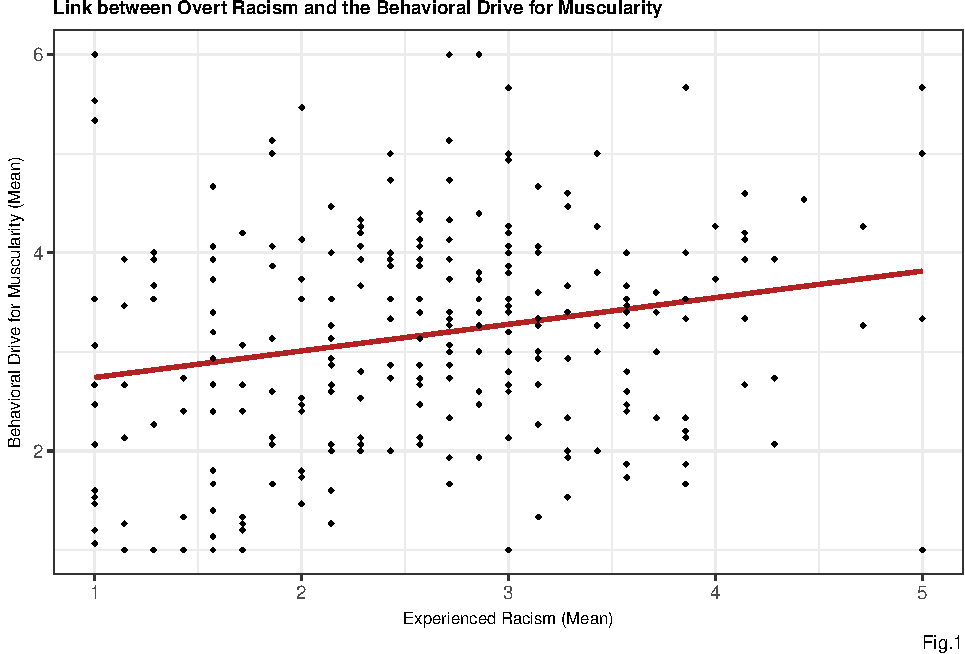
\includegraphics{final_project_files/figure-latex/ggplot-1.pdf} 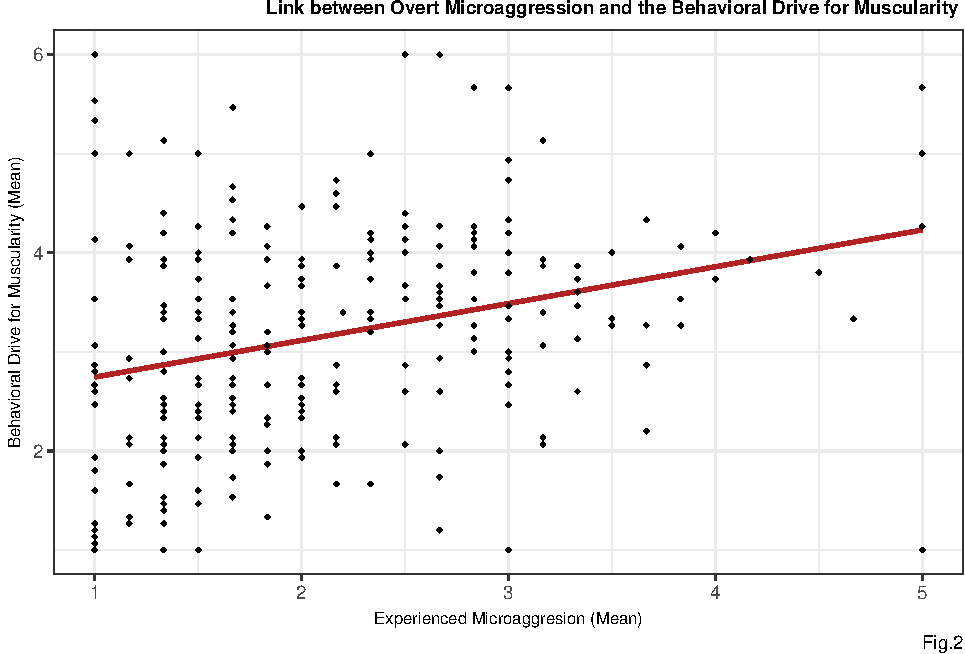
\includegraphics{final_project_files/figure-latex/ggplot-2.pdf}

\hypertarget{discussion}{%
\section{\texorpdfstring{\textbf{Discussion}}{Discussion}}\label{discussion}}

This was the first known study to examine the link between Asian/Asian American men's experiences with race-related discrimination, both in the forms of overt racism and microaggressions, and the behavioral drive for muscularity. As hypothesized, both experiences with overt racism (e.g., ``You see a TV commercial in which an Asian character speaks bad English and acts subservient to non-Asian characters'') and microaggressions (e.g., ``Someone asks you if you can teach him or her karate'') were significantly and positively associated with the behavioral drive for muscularity (e.g., engaging in behaviors aimed at increasing muscle mass).
The current study sheds further light on the harmful effects of racism on Asian/Asian American's mental health, including body image and disordered eating behaviors. This is particularly pervasive given the increasingly muscular, mesomorphic male body ideal perpetuated throughout Western media (Edwards et al., 2016). Extant data suggest that Asian/Asian American men are often stereotyped to be smaller, more feminine, less masculine, and less sexually attractive than their non-Asian peers (Wilkins et al., 2011). As such, it is theorized that when Asian/Asian American men experience race-related discrimination (e.g., overt racism and/or microaggressions), their Asian identity becomes particularly salient, therefore perpetuating internalized feelings of perceived inadequacy with regards to embodying the mesomorphic, Western male body ideal. This, in turn, may result in Asian/Asian American men going to extreme lengths to achieve the ideal body physique, including excessive and compulsive muscularity-enhancing behaviors.
It is important to consider limitations to the current study, including the cross-sectional study design. The findings are correlational, rather than causal, and experimental and prospective data are needed to determine if experiences with racism prompt muscularity-enhancing behaviors. While the current study includes a large, nationally represented sample of Asian/Asian American men, we were underpowered to examine whether the link between experiences with race-related discrimination and muscularity-enhancing behaviors vary by Asian ethnic identity (e.g., Chinese, Japanese, Korean, Asian Indian, Filipino, and other Asian subgroups). Future research should seek to clarify whether there are intra- and inter-ethnic variations in these associations.
Although prospective and mechanistic studies are needed, these findings indicate that experiences with race-related discrimination negatively impact Asian/Asian American men's body image, thus prompting engagement in potentially harmful and compulsive muscularity-enhancing behaviors. The current study adds to a small, but growing body of research implicating experiences with race-related discrimination as a significant contributor to health disparities among racial/ethnic minority men living in the United States. These data may help to inform clinical programming and preventative interventions aimed at addressing the harmful effects of race-related discrimination on men's body image and disordered eating behaviors. The current study may also help to inform the development and implementation of interventions aimed at helping Asian/Asian American men adopt healthy coping strategies in response to discriminatory experiences. Overall, this study sheds light on the numerous, adverse effects of race-related discrimination on minority mental health.

\newpage

\hypertarget{references}{%
\section{References}\label{references}}

\begingroup
\setlength{\parindent}{-0.5in}
\setlength{\leftskip}{0.5in}

\hypertarget{refs}{}
\begin{CSLReferences}{0}{0}
\end{CSLReferences}

\endgroup


\end{document}
